\documentclass[10pt,a4paper,twoside]{article}
% The following LaTeX packages must be installed on your machine: amsmath, authblk, bm, booktabs, caption, dcolumn, fancyhdr, geometry, graphicx, hyperref, latexsym, natbib

% Please make sure that spp.dat (supplied with this template) is in your working directory or path
\input{spp.dat}

%  Editorial staff will uncomment the next line
% \providecommand{\artnum}[0]{XX-XX}
% \renewcommand{\articlenum}[0]{SPP-\the\year-\artnum-}

\begin{document}

%--------------------------------------------------
%  Fill in the paper's title in Sentence case
%  Titles beginning with articles (A, An, The) are discouraged
%--------------------------------------------------
\title{\TitleFont Learning dynamics in a cellular automata model of classroom peer-to-peer interactions}


%--------------------------------------------------
% For TWO authors with the same affiliation please use this block
% Or Please use the other author block templates
%--------------------------------------------------
\author[*\negthickspace]{Clarence Ioakim T.~Sy}
\author[ ]{Johnrob Y.~Bantang
\lastauthorsep}
\affil[ ]{National Institute of Physics, University of the Philippines - Diliman, Philippines}
\affil[*]{\corremail{csy@nip.upd.edu.ph} }

%--------------------------------------------------
%  For three or more authors with the same affiliation please use this block
%--------------------------------------------------

% \author[*]{Author M.~Surname\authorsep}
% \author[ ]{Bauthor D.~Surname~Jr.\authorsep}
% \author[ ]{Cauthor D.~Surname~III\lastauthorsep}
% \affil[ ]{Department of Science, XXX University, Country}
% \affil[*]{\corremail{amsurname@university.edu} }

%--------------------------------------------------
%  For authors with different affiliations please use the following block
%--------------------------------------------------
% \author[1*]{Author M.~Surname\authorsep}
% \author[2]{Bauthor D.~Surname~Jr.\authorsep}
% \author[1,2]{Coauthor G.~Surname~III\authorsep}
% % !!! Please take note that the last author separation is \lastauthorsep instead of \authorsep
% \author[3]{Dauthor G.~Surname\lastauthorsep}
% \affil[1]{Department of Physics, DD University, Country}
% \affil[2]{Department of Science, XX University, Country}
% \affil[3]{Physics Institute, Country}
% \affil[*]{\corremail{amsurname@university.edu} }


\begin{abstract}
\noindent
%--------------------------------------------------
% Include abstract and keywords here
%--------------------------------------------------
This study aims to model the transfer of knowledge through peer-to-peer interactions in the classroom by using a binary probabilistic cellular automata (PCA) model. This study mainly focuses on the effects of the  initial seating arrangement of learned or high aptitude students to the classes' overall learning rate. We found that in square classrooms with different lengths $L \in\lbrace32,64,128\rbrace$, the inner corner seating arrangement performed the best in terms of both time it takes to saturate the classroom with learned students ($T$) and the classroom’s learning rate in the first half of the simulation before the finite size effect affects the system ($m$). This result is different from a similar previous study by Roxas et. al. (2010). This difference stems from the simplifications made in this model. Our model uses binary values instead of continuous values as a measure of students’ aptitude, does not consider directionality or orientation bias (non-isotropy), the similarity effect mentioned in related literature (?), and does not incorporate memory or unlearning - all of which are factors in the real world.

\keywords{classroom dynamics, probabilistic cellular automata}

\end{abstract}

\maketitle
\thispagestyle{titlestyle}


%--------------------------------------------------
% the main text of your paper begins here
%--------------------------------------------------
\section{Introduction}\label{sec:intro}


\section{Methodology}\label{sec:methods}
We used a two-dimensional binary probabilistic cellular automata (PCA) model to simulate the learning of students from peer-to-peer interactions in a classroom. The PCA model parameters include: (1) spread coefficient matrix $\Lambda$ (eq \ref{eq:Lambda matrix}) in a neighborhood which can be both isotropic (no orientation bias, all $\lambda_i$ are equal) and anisotropic (has orientation bias, not all $\lambda_i$ are equal), (2) the dimensions of the classroom ($L_1 \times L_2$) such that the size is $N=L_1 \times L_2$, and (3) the initial position of the learned students. The initial positions chosen for the simulations are based on a previous study from Roxas et. al. (2010) \cite{roxas2010seating}, namely inner corner, outer corner, center, and random with the number of initial learned students being constantly $n_0 = 4$. 

\begin{equation}\label{eq:Lambda matrix}
  \Lambda = 
  \begin{bmatrix}
  \lambda_1 & \lambda_4 & \lambda_7\\
  \lambda_2 & \lambda_5 & \lambda_8\\
  \lambda_3 & \lambda_6 & \lambda_9\\
  \end{bmatrix}, \text{where } \lambda_i=\lambda \forall i \in \lbrace1...9\rbrace
\end{equation}

\noindent In the simulations ran for this experiment, only isotropic spreading was considered with spread coefficients ($\lambda$) between 0.1 to 1.0 with increments of 0.1. The matrix $\Lambda$ dictates the probability of the student of interest, placed at the center of the matrix, to learn from its neighbors based on the latter's relative position. For example, an unlearned student whose only learned neighbor is in front of them will have a $\lambda_4$ chance of learning in the next generation. The probability of an unlearned student learning from multiple neighbors is dictated by equation \ref{eq:learning probability}.

\begin{equation}
  P = 1 - \prod_{n=1}^{9}{(1-S_n\lambda_n)}
  \text{, where } S_n=
  \begin{cases}
    0 & \text{when neighbor is learned}\\
    1 & \text{when neighbor is not learned}
  \end{cases}
  \label{eq:learning probability}
\end{equation}

\noindent The classrooms were set to be squares with lengths $L \in \lbrace 32,64,128\rbrace$. This is not representative of reality and it was done because a classroom length of 8 (and corresponding size of 64) will not give much insight as the simulations would end too quickly and would not have yielded enough data points for analysis.

\subsection{Time to learn and learning rate}
From the simulations, we compared both the average number of generations it takes to saturate the classroom with learned students ($T$) and the average learning rate across different configurations over 5 independent runs. The learning rate for each trial was obtained by fitting a power model ($y = ax^m$) to the first half of the data, which is often before the finite size effect starts to affect the simulation, and taking the exponent as the characteristic variable or learning rate ($m$) for that independent run.


\subsection{Size dependence}
We also analyzed the dependence of the time to learn ($T$) on the class size ($L^2$). For each seating arrangement, we took representative learning coefficients $\lambda \in \lbrace 0.1, 0.5, 0.9 \rbrace$ to see how the class size and the learning coefficient affects the time to learn.

\section{Results and Discussion}
The data shown in Figure \ref{fig:TTL and m vs lambda} suggests that the time to learn ($T$) (\textit{Plot labels not yet corrected}) does not vary significantly between the outer corner, center, and random seat configurations across classroom sizes and spread coefficients. However, there is a significant difference between random arrangement when compared against the outer corner and inner corner seating arrangements. The inner corner seating arrangement consistently performs the best with the shortest time to saturate the classroom with learned students ($T$) and the highest characteristic variable or learning rate ($m$), while the random arrangement generally performs the worst. These findings can be attributed to the simplicity of the model which lends itself to being heavily influenced by geometric factors. Analytically, the configurations’ performance is dictated by the maximum distance of any point to an initially learned student. The outer corner and center seating arrangements perform very similarly because they are geometrically one circle expanding at a constant rate. In these two configurations, the maximum distance of any unlearned student to an initially learned student is the same at $d_{\text{max, center}} = d_{\text{max, outer corner}}=\frac{L\cdot\sqrt{2}}{2}$. The inner corner seating arrangement performs the best because it minimizes this distance to $d_{\text{max, inner corner}}=\frac{L\cdot\sqrt{2}}{4}$.

%figures of lambda dependence
\begin{figure}[h!]
  \centering
  \subfloat{\makebox[0.3\textwidth]{{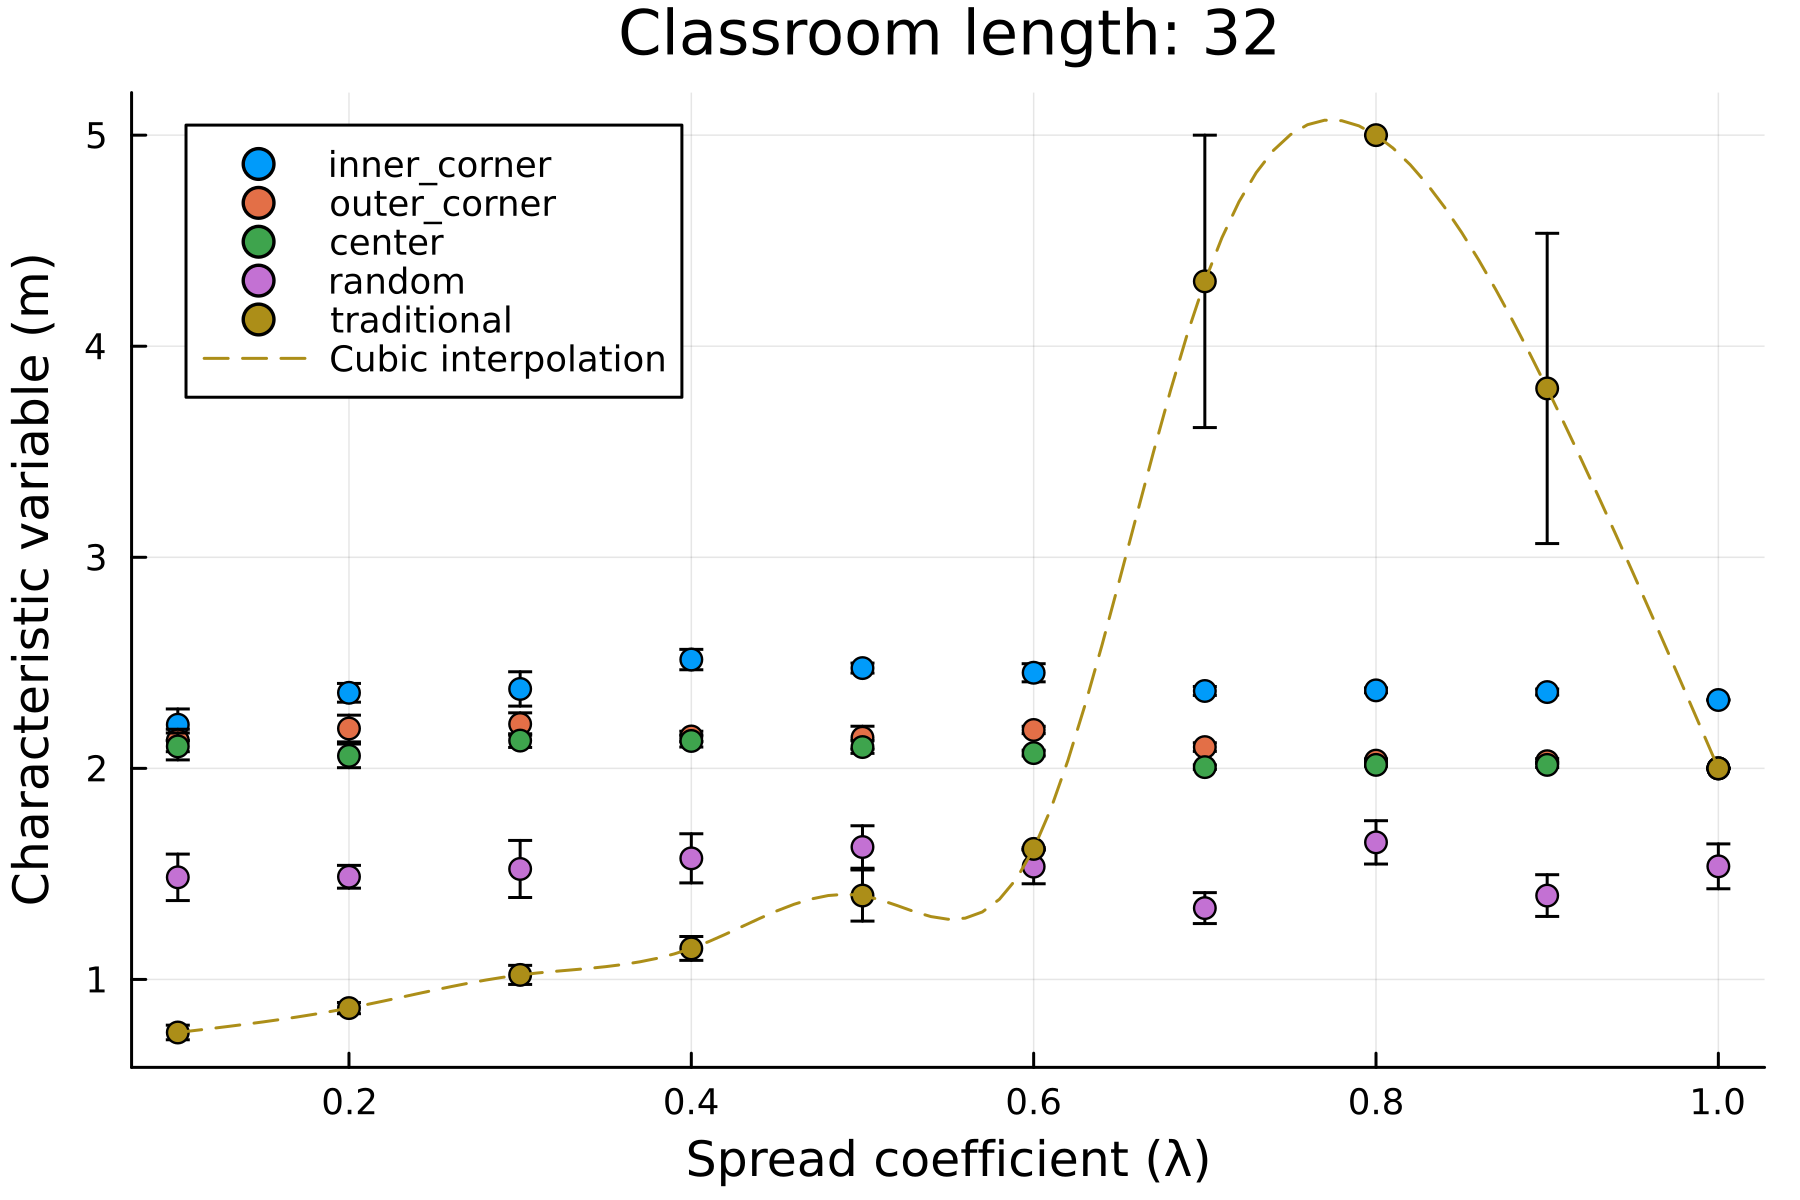
\includegraphics[width=0.3\textwidth]{figures/m-32.png}\label{fig:m-32}}}}
  \quad % or other spacing between figures
  \subfloat{\makebox[0.3\textwidth]{{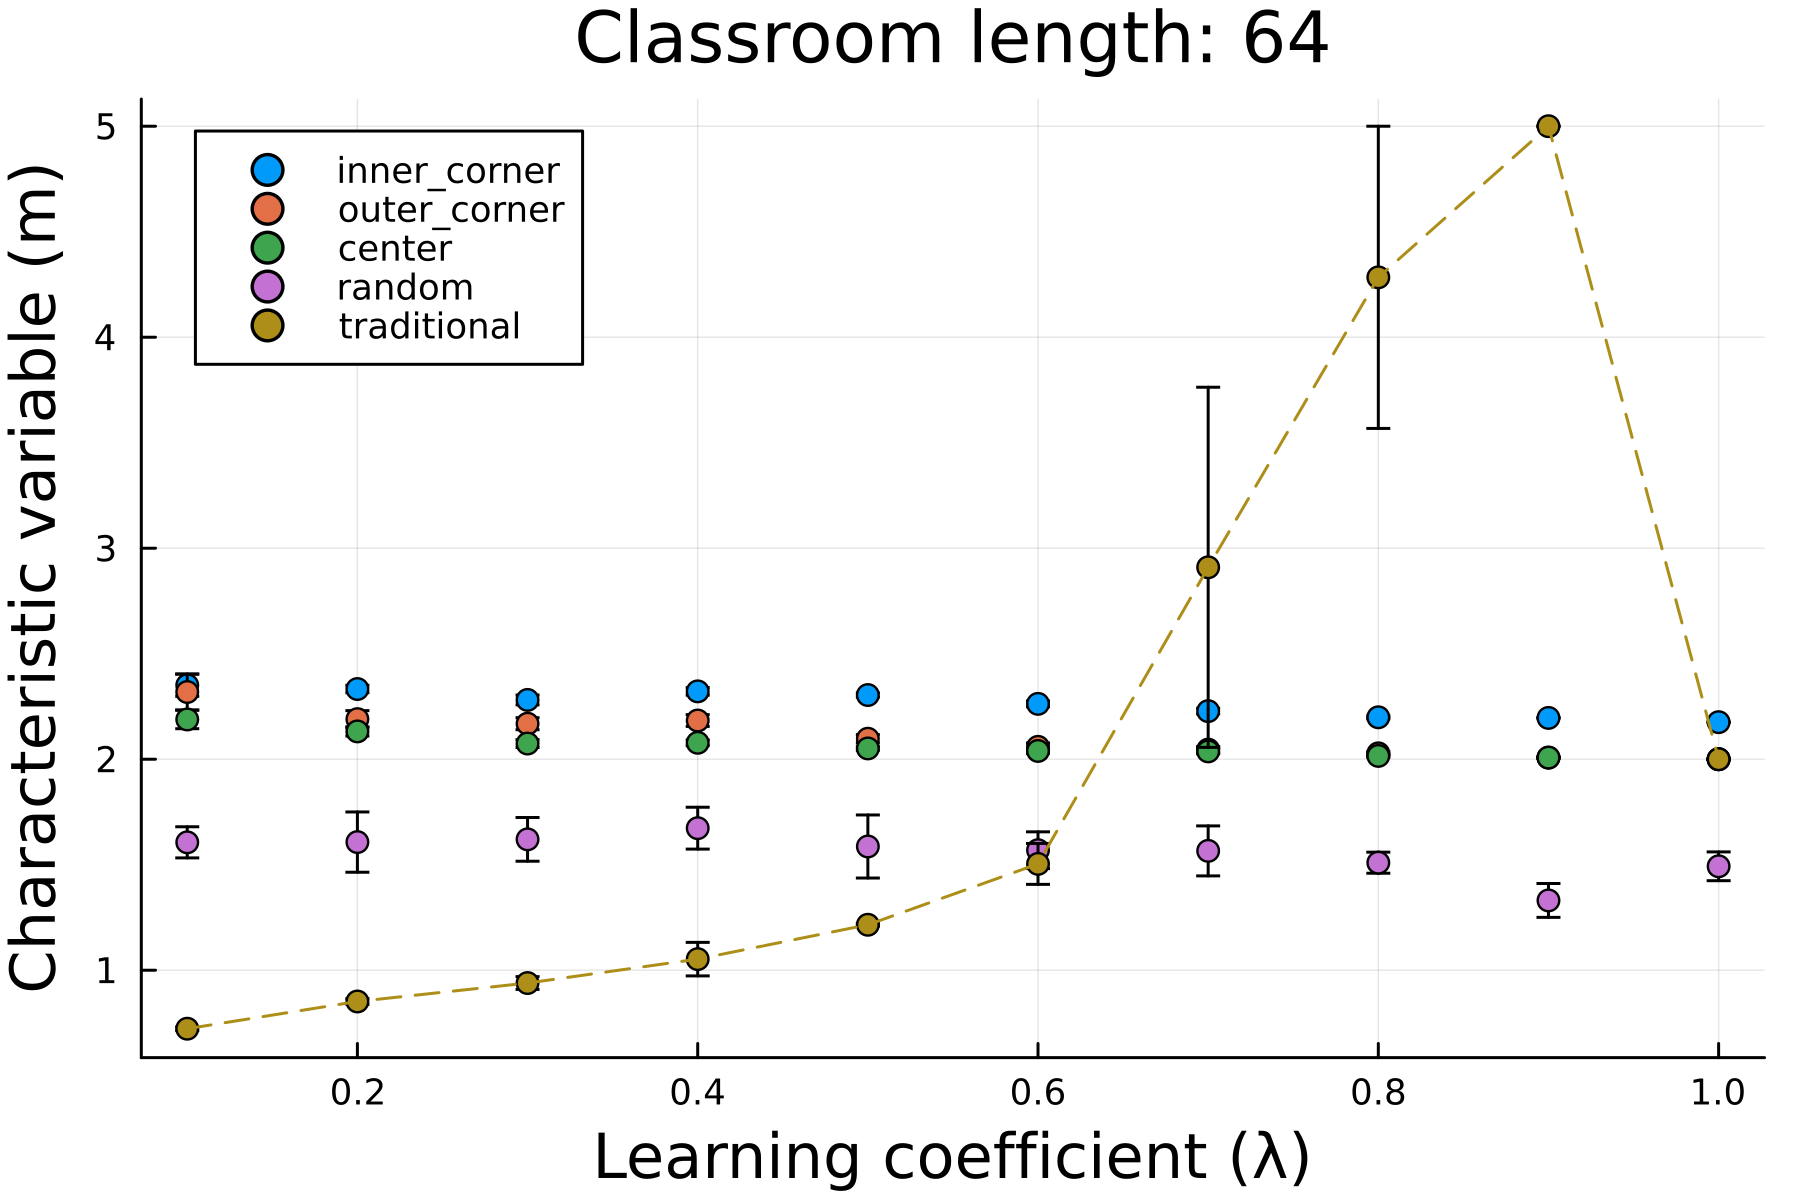
\includegraphics[width=0.3\textwidth]{figures/m-64.png}\label{fig:m-64}}}}
  \quad % or other spacing between figures
  \subfloat{\makebox[0.3\textwidth]{{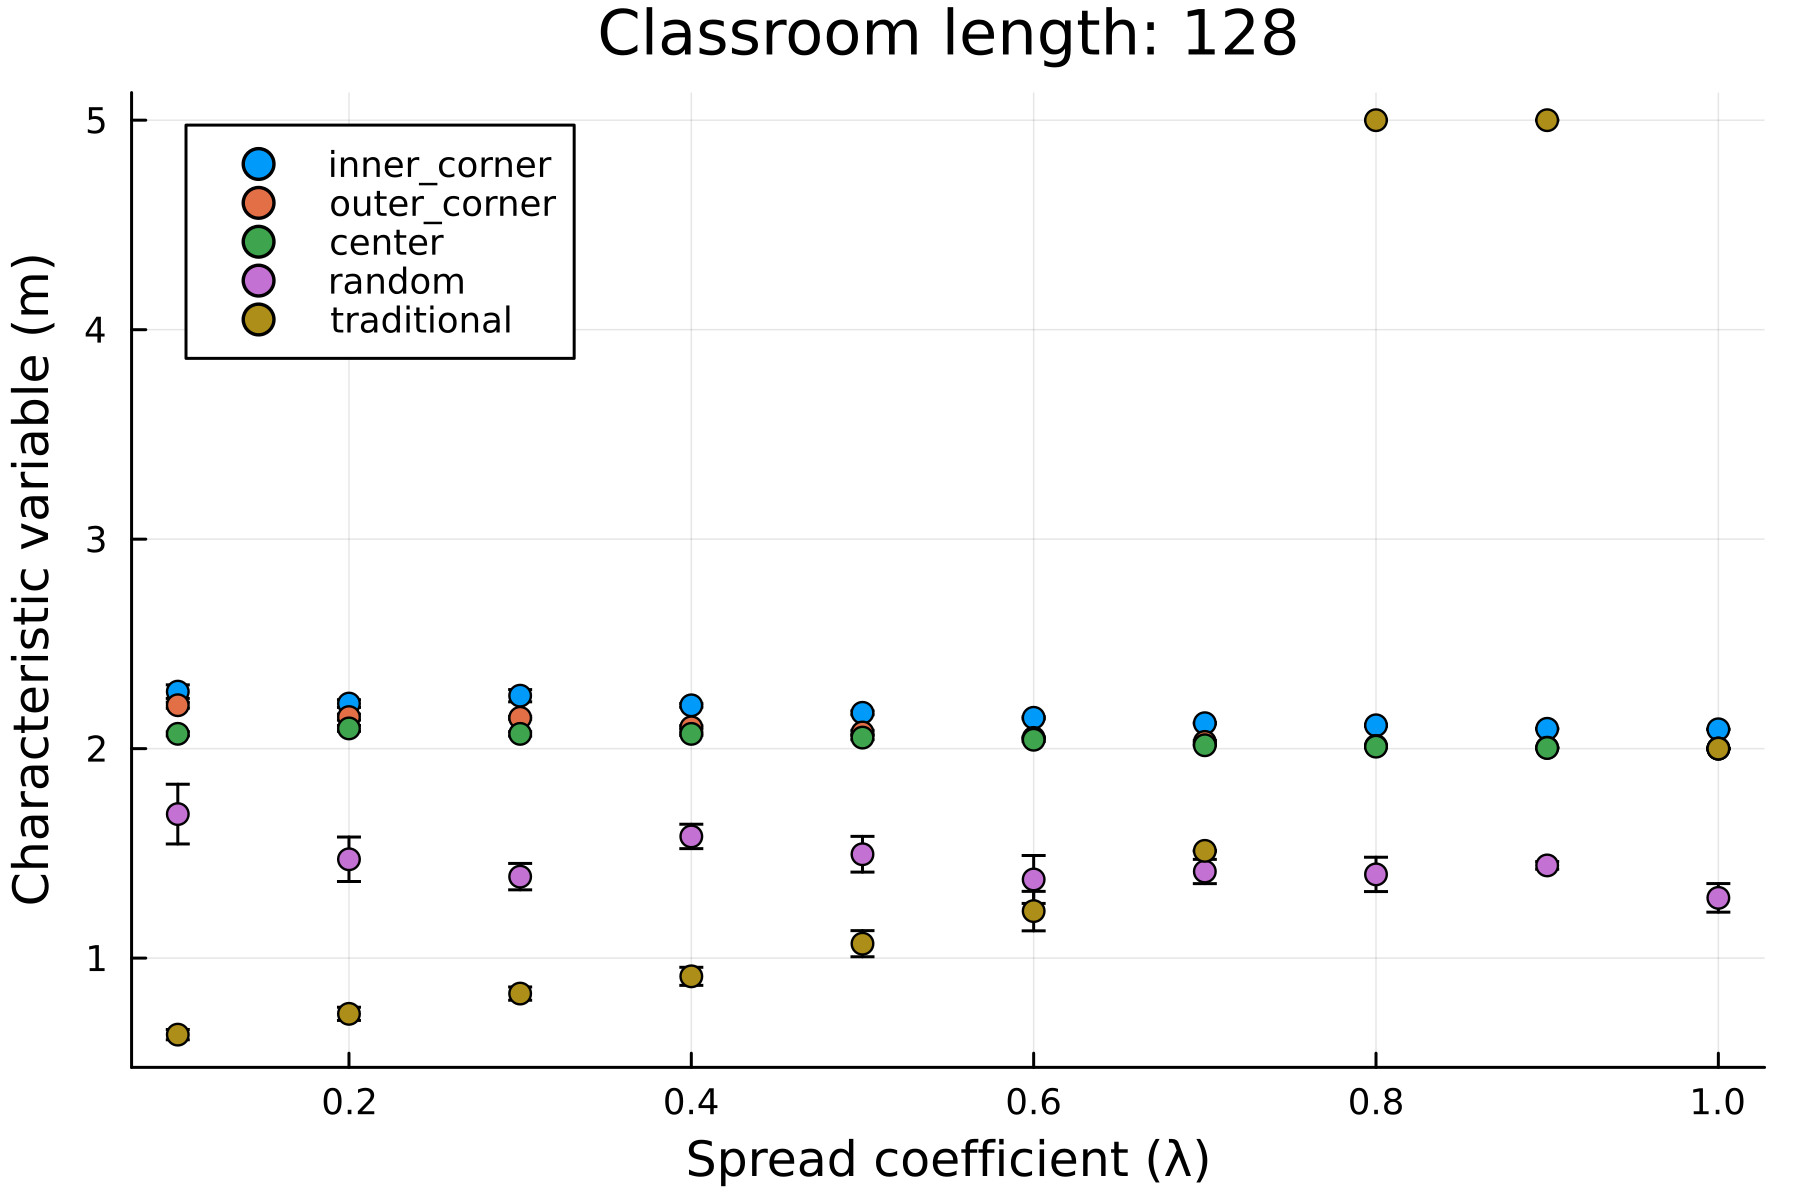
\includegraphics[width=0.3\textwidth]{figures/m-128.png}\label{fig:m-128}}}}
  \quad % or other spacing between figures
  \subfloat{\makebox[0.3\textwidth]{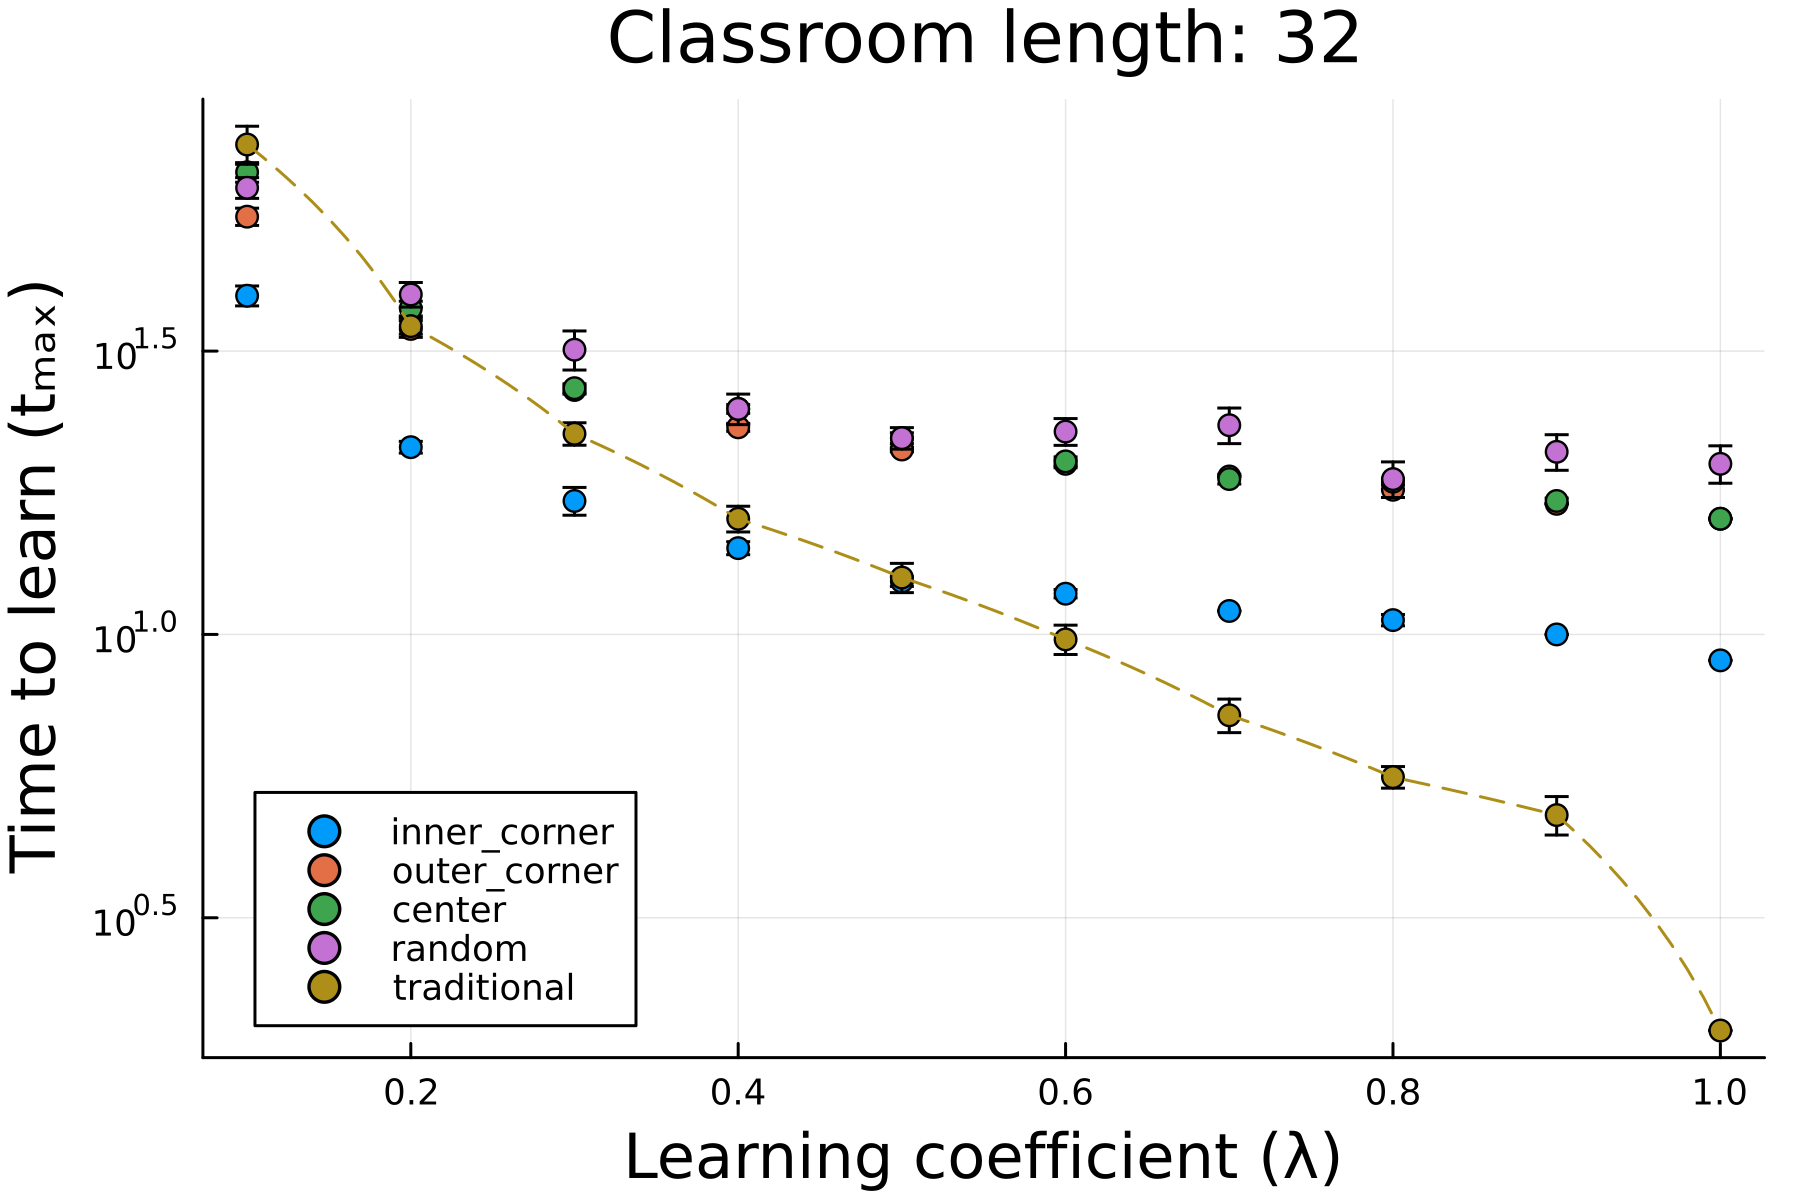
\includegraphics[width=0.3\textwidth]{figures/t-32}\label{fig:t-32}}}
  \quad % or other spacing between figures
  \subfloat{\makebox[0.3\textwidth]{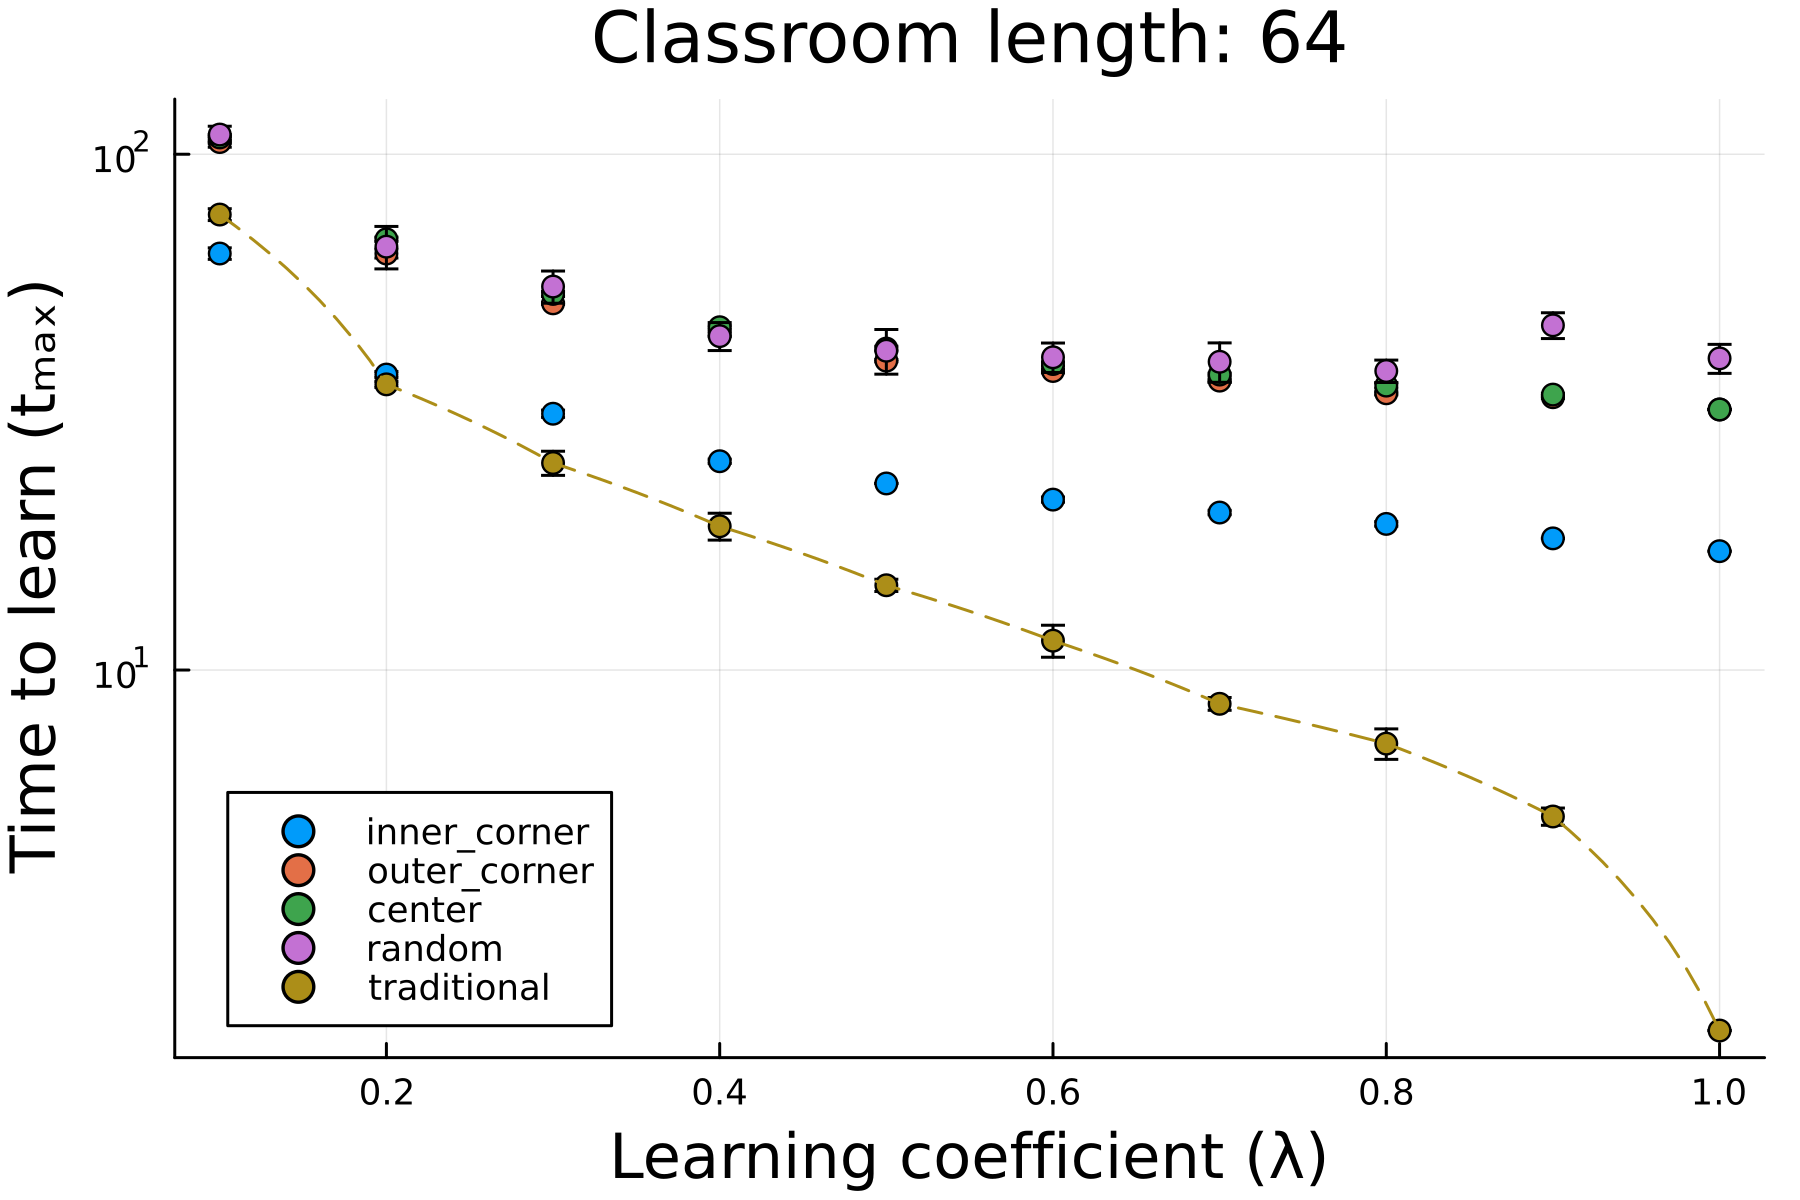
\includegraphics[width=0.3\textwidth]{figures/t-64}\label{fig:t-64}}}
  \quad % or other spacing between figures
  \subfloat{\makebox[0.3\textwidth]{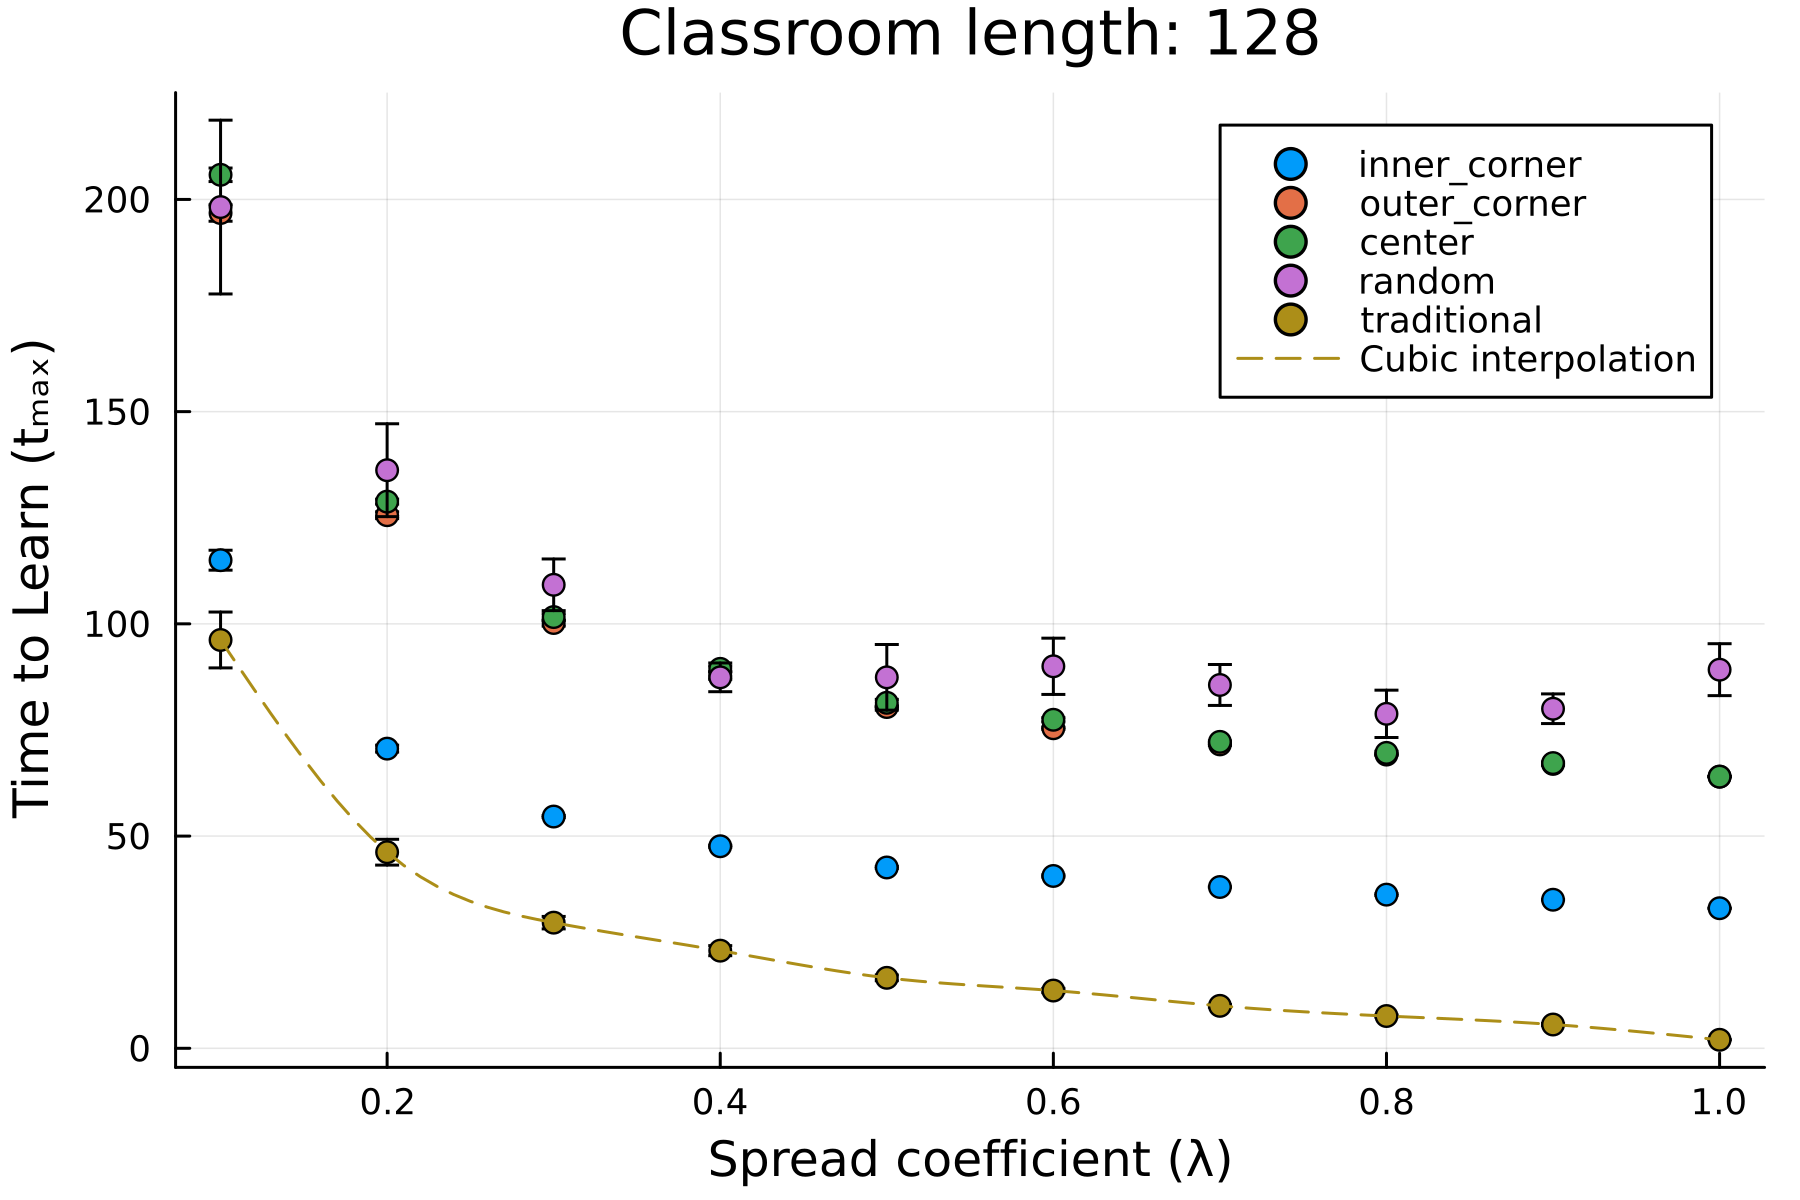
\includegraphics[width=0.3\textwidth]{figures/t-128}\label{fig:t-128}}}
  \caption{Characteristic variable ($m$) and time to learn ($T$) vs. Spread coefficient ($\lambda$).}\label{fig:TTL and m vs lambda}
\end{figure}

\noindent These results, however, do not agree with existing studies. In a similar study by Roxas et. al. (2010) \cite{roxas2010seating}, they found that the outer corner configuration performed the best in reality. The difference is expected due to the simplifications made in this study. They mentioned that there is a similarity effect that goes on in peer-to-peer learning wherein students of the the same aptitude level, regardless of their actual aptitude, learn better when seated together. The similarity effect has not yet been implemented in our system because this is not applicable to a binary system. The system being binary also introduces more granularity when compared to reality where aptitude is measured more continuously. This study also does not consider the non-isotropy or the presence of an orientation bias when it comes to the learning within each neighborhood. Non-isotropy in the system can stem from the fact (citation needed?) that students may prefer to interact with students beside them or in front of them instead of behind them out of convenience, possibly leading to more learning. This study also assumes that everyone is equally receptive to learning from their peers which may not be the case, so future models will/should take into account the non-uniformity of individuals’ learning rates. 

%figure of TTL vs Size
\begin{figure}[h!]
  \centering
  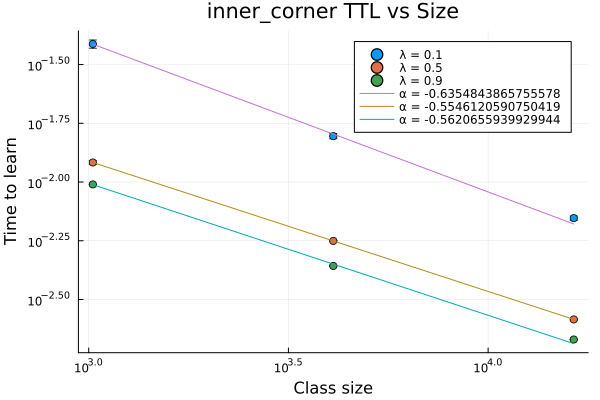
\includegraphics[width=0.4\textwidth]{figures/scale_factor_preadjusted.png}
  \caption{Time to Learn ($T$) vs Class size ($L^2$)}
  \label{fig:scale factor unadjusted}
\end{figure}

\noindent The linear plot on the log-log scale in Figure \ref{fig:scale factor unadjusted} (\textit{plot labels and legend not yet fixed}) suggests that the relationship of the time to learn vs class size is dictated by a power law wherein it can be normalized so that the lines would collapse. (\textit{no plot yet})
\\
\\
\section{Conclusions}
Here is the Summary or Conclusions section.

\section*{Acknowledgments}
Here are the acknowledgments. Note the asterisk \textbackslash{\ttfamily section*}\{{\ttfamily Acknowledgments}\} that signifies that this section is unnumbered.

% Please use the style file spp-bst.bst. If you wish to use BibTeX, kindly use us the filename bibfile.bib for your bib file.
\bibliographystyle{spp-bst}
\bibliography{bibfile}

\end{document}